\newpage

\section{Problem}
Software availability is a crucial determinant in the acceptance and implementation of technology among individuals and organizations. One significant aspect of software availability is the compatibility of the operating system (OS) with the software, which determines whether the software can be installed and utilized on a specific OS. In recent years, Linux has gained popularity among users and organizations due to its open-source nature, security, and flexibility.

Within our university, several training rooms utilize KVM-Switches, which come equipped with management software available exclusively for Windows and Mac operating systems. To address this issue, we undertook the task of reverse engineering the switching signal of these KVM Switches and developing a script compatible with Linux systems.

\subsection{Device}
The apparatus under consideration is a Uniclass UDP-TA2-4K KVM Switch, as illustrated in Figure 1. This device presents the capability to interconnect two computers utilizing a single monitor, mouse, and keyboard. The preferred computer can be chosen through a hardware button, which is a wired remote control, or via the KVM Switching Software.

\begin{figure}[htp!]
    \centering
    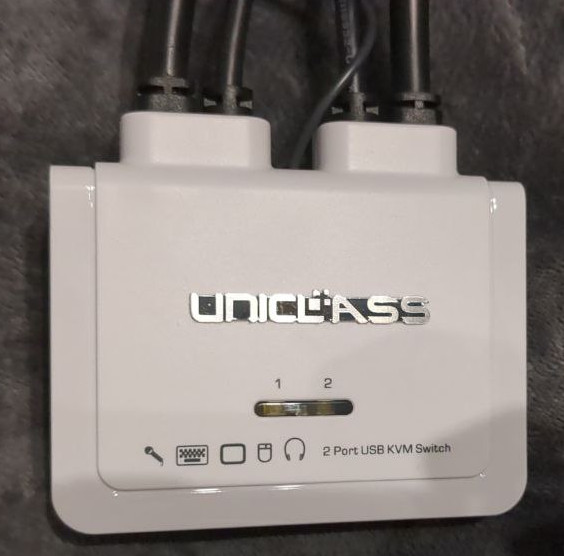
\includegraphics[width=11cm]{img/device.jpg}
    \caption{UDP-TA2-4K KVM Switch}
    \label{fig:UDP-TA2-4K KVM Switch}
\end{figure} 

\subsection{Software}
The management software for Windows and MAC PCs can be found on the product webpage of Uniclass \cite{Uniclass_Webpage}. The software can be operated via hotkeys. It is crucial to note that the KVM Switch requires both output-ends to be connected to a computer; otherwise, the software will not function. The USB and Displayport connections are verified during setup.

The Windows Software was utilized to manage the KVM Switch, providing a tray icon where users can control the two displays, if connected, and access the "Settings" menu. Where we did not utilize the "Advanced Options" section. In the "Hot Key To Switch To" option, users can modify the Hot-Key settings to switch between the two output-ends. By default, the switching keys are "CTRL + ALT + 1" for PC1 and "CTRL + ALT + 2" for PC2.


\section{Analysis}
\subsection{Preparation}
We will analyze USB traffic using Wireshark. To enable Wireshark-USBPcap on Linux, execute the following commands:
\begin{lstlisting}[language=Bash, basicstyle=\small]
sudo apt-get install wireshark libpcap0.8
sudo modprobe usbmon
sudo setfacl -m u:$USER:r /dev/usbmon*
\end{lstlisting}

\subsection{Investigate}
The aim of this study is to document the relationship between the device and the software. Initially, the primary challenge encountered was identifying the appropriate port to which the device was connected.A good resource about USB can be found here \cite{Beyond_Logic}. Following this, it was observed that a small number of packages (18-30) consistently appeared at the start of Wireschark/USBPcap.

\begin{figure}[htp!]
    \centering
    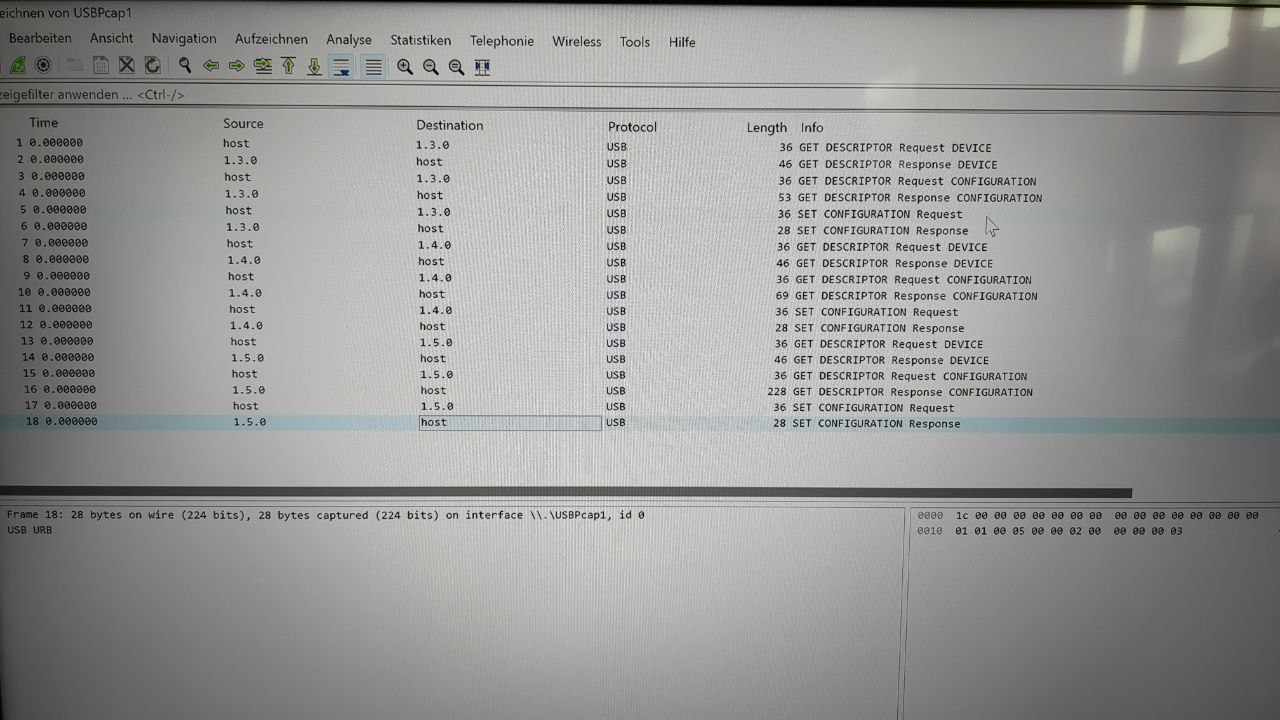
\includegraphics[width=11cm]{img/pre_sniff.jpg}
    \caption{Screenshot Wireshark Start-Packages}
    \label{fig:Screenshot Wireshark Start-Packages}
\end{figure}

A capture was generated during the switching of the KVM Switch, and has been saved in the file "signal.pcapng".

\begin{figure}[htp!]
    \centering
    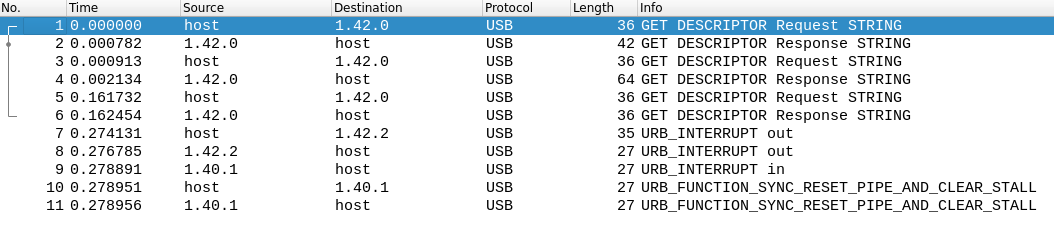
\includegraphics[width=11cm]{img/signal.png}
    \caption{Screenshot Wireshark signal.pcapng}
    \label{fig:Screenshot Wireshark signal.pcapng}
\end{figure}

During the initial six connections, there is an exchange of product information and configurations. Notably, the device name "2Port KVMSwitcher" is transmitted in ASCII string format, which provides insight into the identity of the device. It is also presumed that information regarding the state of the KVM Switch is communicated during this phase. The seventh request is of particular significance, as it involves the transmission of the command to alter the device state. This is accomplished via the "URB\_INTERRUPT" out with Leftover Capture Data 0101000000000000 at Endpoint 0x02. The specific data transmitted varies depending on the current state of the device.

\begin{figure}[htp!]
    \centering
    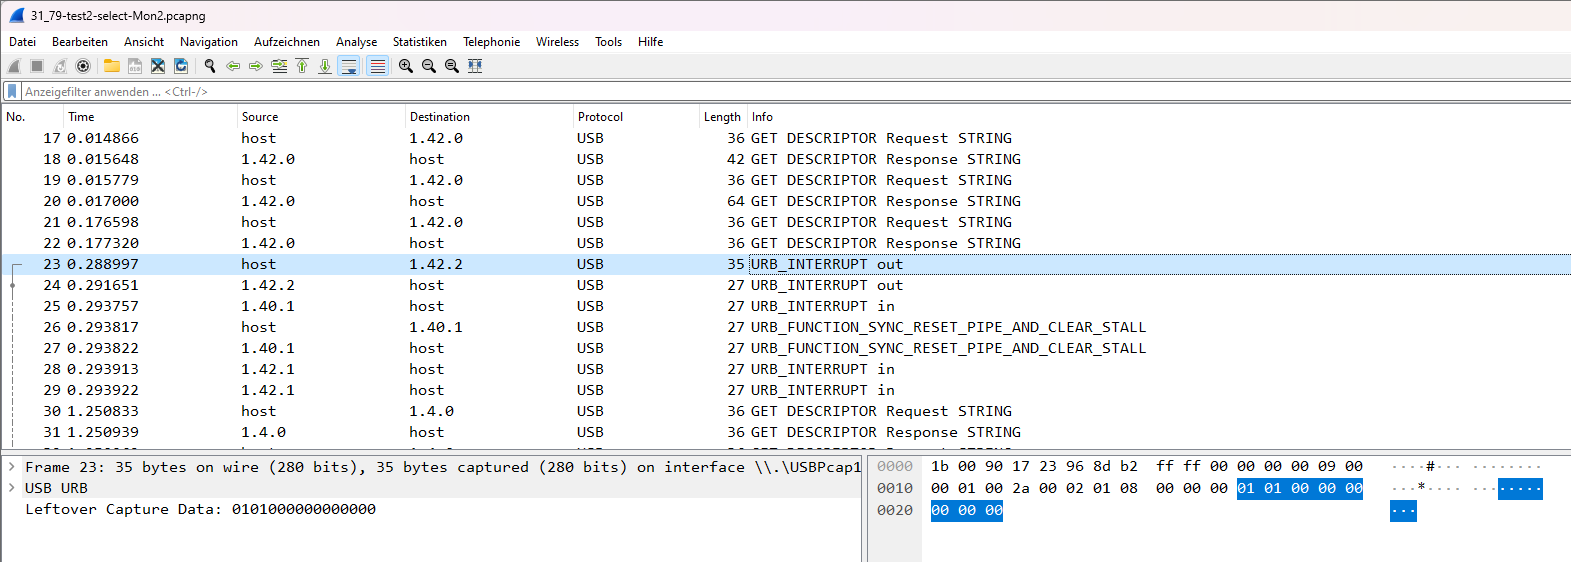
\includegraphics[width=11cm]{img/packet_1_2.png}
    \caption{Screenshot Wireshark State 0101000000000000}
    \label{fig:Screenshot Wireshark State 0101000000000000}
\end{figure}

\begin{figure}[htp!]
    \centering
    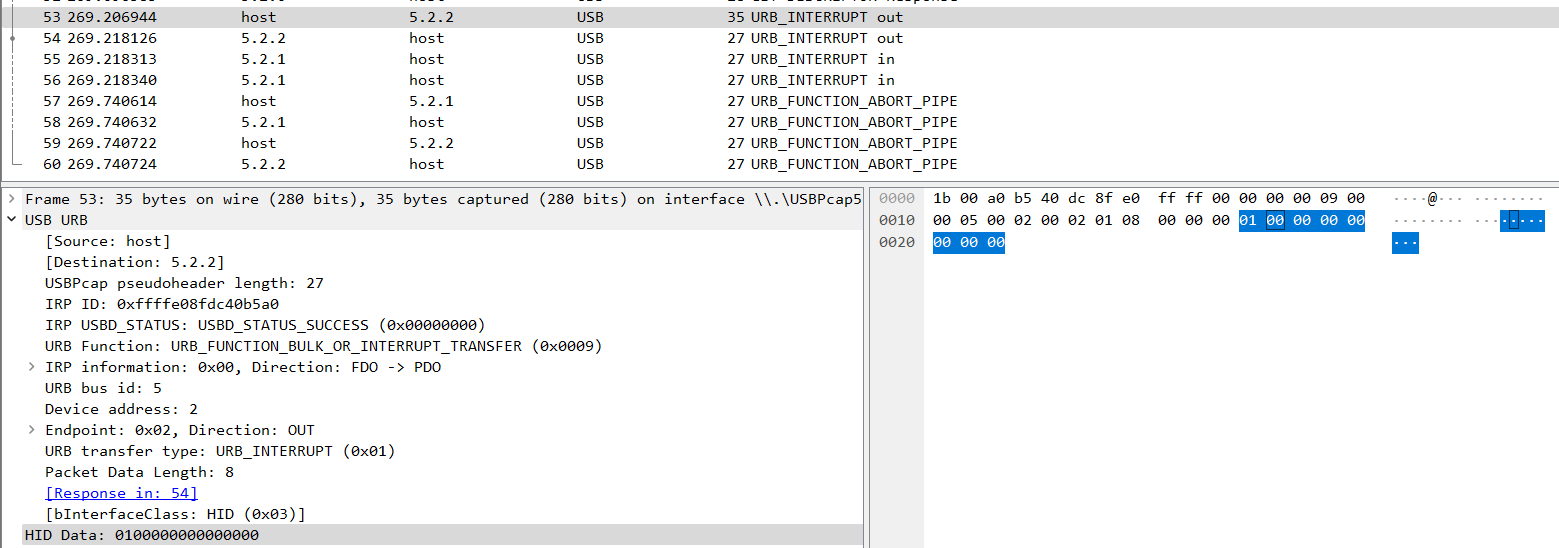
\includegraphics[width=11cm]{img/packet_2_1.png}
    \caption{Screenshot Wireshark State 0100000000000000}
    \label{fig:Screenshot Wireshark State 0100000000000000}
\end{figure}

Following the computer's request, the device responds with an "URB\_INTERRUPT out", serving as a confirmation. Subsequently, the device transmits "URB\_INTERRUPT in", the purpose of which remains unknown and seemingly inconsequential. Finally, the URB Function Abort PIPE is observed, which we hypothesize to be the conclusive signal of termination.

\section{Solution}
\subsection{Preparation}
In order to transmit data or packets to a USB device, Python can be utilized. To install the necessary software, the following instructions must be followed:

\begin{lstlisting}[language=Bash, basicstyle=\small]
sudo apt install python3 python3-pip
sudo python3 -m pip install pyusb
\end{lstlisting} 

\  \\

Use "lsusb" to get information from the Device:
\begin{lstlisting}[language=Bash, basicstyle=\small]
Bus 002 Device 004: ID 10d5:55a2 Uni Class Technology Co., Ltd 2Port KVMSwitcher
\end{lstlisting}
The Vendor Id is 0x10d5 the Product Id is 0x55a2.

\subsection{Sending Data to USB}
We have developed a Python script, utilizing PyUSB\cite{PyUSB}, which facilitates data transmission to the USB port through send.py. The primary objective is to dispatch "URB\_INTERRUPT out".

\begin{lstlisting}[language=Python,numbers=left, basicstyle=\small]
#!/usr/bin/python
import sys
import usb.core

dev = usb.core.find(idVendor=0x10d5, idProduct=0x55a2)

print(dev)
dev.write(ENDPOINT, 'TEXT')
\end{lstlisting}

It took some work to model the signal in Python so that the switch reacts to it.

\subsection{First switching script}
In order to transmit information in bytecode format, a bytearray \cite{Programiz/python-programming} was constructed, which was subsequently decoded into a string \cite{python_docs} \cite{Stackoverflow}. This step was necessary due to the syntax of the dev.write instruction, which mandates the transmission of information in string format to the USB device. Further information on the conversion process was obtained from the source cited herein.

\begin{lstlisting}[language=Python,numbers=left, basicstyle=\small]
#!/usr/bin/python
import usb.core

dev = usb.core.find(idVendor=0x10d5, idProduct=0x55a2)

if dev is None:
    raise ValueError('KVM-Switch not connected!')
else:
    print('KVM-Switch found.')

payload_1_2 = bytearray([1, 1, 0, 0, 0, 0, 0, 0])
payload_2_1 = bytearray([1, 0, 0, 0, 0, 0, 0, 0])

try:
    dev.write(2, payload_2_1.decode('utf-8'))
    dev.write(2, payload_1_2.decode('utf-8'))
except:
    print('success!')
\end{lstlisting}

\subsection{Finishing the script}
In order to finalize the script, it was necessary to identify the appropriate endpoint for transmitting the required bytecode for executing the switching command. This endpoint was determined by examining lines 17 and 24 of switch\_with\_state.py. If endpoint 02 was encountered, an error occurred, prompting the implementation of an error handling mechanism (lines 18-21).
\newpage
\begin{lstlisting}[language=Python,numbers=left, basicstyle=\small]
#!/usr/bin/python
import usb.core
import usb.util

payload_1_2 = bytearray([1, 1, 0, 0, 0, 0, 0, 0])
payload_2_1 = bytearray([1, 0, 0, 0, 0, 0, 0, 0])

dev = usb.core.find(idVendor=0x10d5, idProduct=0x55a2)

if dev is None:
    raise ValueError('KVM-Switch not connected!')
else:
    print('KVM-Switch found.')

serial_number = usb.util.get_string(dev, dev.iSerialNumber)

if (serial_number.encode('utf-8')) == b'02\xc2\x92':
    try:
        dev.write(2, payload_1_2.decode('utf-8'))
    except:
        pass
    print ("switched from 1 to 2")

if (serial_number.encode('utf-8')) == b'12\xc2\xb2':
    dev.write(2, payload_2_1.decode('utf-8'))
    print ("switched from 2 to 1")
\end{lstlisting}

\section{Executive Summary}
In summary, it can be stated that the regression of the USB signal has been successful. The process has been translated into a Python script, which is now compatible with Linux operating systems and can be executed accordingly.
